\subsection{\gjets and QCD multijet estimation}   

Along with the presence of a well identified high \pt photon in the event, the \gjets production contributes to the background in search regions if one of the jets in an event is mis-measured resulting in fake \ptmiss or it contains a jet originating from b-quarks with a semileptonic decay of B mesons. Fluctuations in hadronization of jets can also result in an energetic $\pi^0$ misidentified as a photon which along with fake \ptmiss originating from other jets in the event can result in a QCD multijet production contribution to the search regions. Fake \ptmiss arising from mis-measurements of jets or semileptonic b-jets is usually aligned with the jet itself. Hence, a most of this background is rejected by angular cuts summarized in section \ref{sec:event-selection} i.e. \dphi(\ptvecmiss, \ptvecjet) $>$ 0.3 for first two leading jets. The main contribution to background is due to the \gjets processes and QCD multijet contribution is very small. In the method described in this section, the total background due to fake \ptmiss is estimated without further separating the QCD multijet and \gjets processes. 
The control sample to estimate the \gjets and QCD multijet background is derived inverting the \dphi(\ptmiss, jet1) and \dphi(\ptmiss, jet2) criteria (min($\dphi_{1},\dphi_{2}$) $<0.3$) while keeping all the search selections intact except that 100 $<$ \ptmiss $<$ 200~\gev sideband is also used.  Since fake \ptmiss and mis-measured jets are mostly aligned in transverse direction, the inverted \dphi region provides a high statistics region rich in multijet background. Figure \ref{fig:supp_Sim_mindPhi1dPhi2_T5bbbbZG} shows the min($\dphi_{1},\dphi_{2}$) distribution in MC with \ptmiss $>200$ \gev. 
\begin{figure}[h!]
\centering
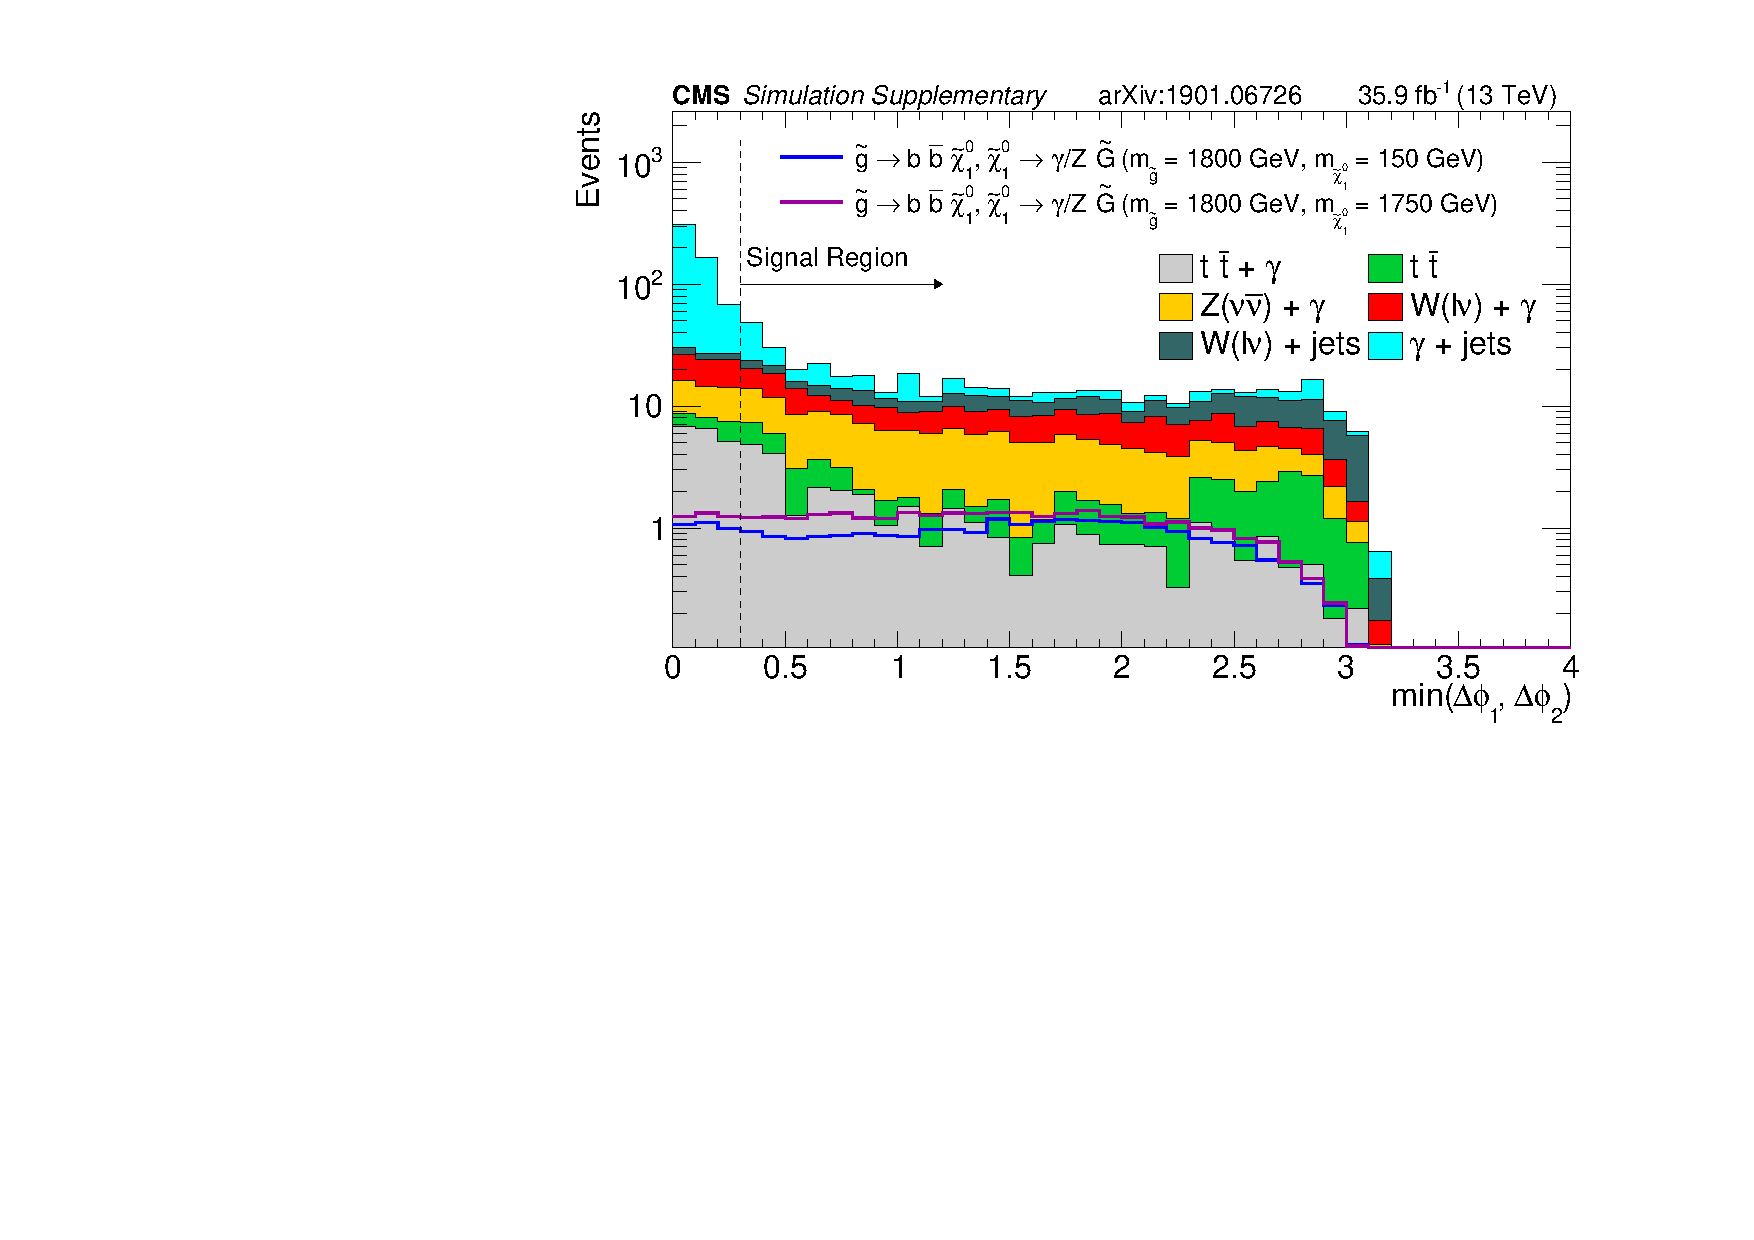
\includegraphics[width=0.8\linewidth]{../Figures/Chap3/anaPublic/supp_Sim_mindPhi1dPhi2_T5bbbbZG}
\captionsetup{width=.9\linewidth}
\caption[Min($\dphi_{1},\dphi_{2}$) in MC]{Distribution of min($\dphi_{1},\dphi_{2}$) in MC after applying all signal region selections except angular cuts. The region min($\dphi_{1},\dphi_{2}$) below 0.3 serves as a \gjets enriched sample and min($\dphi_{1},\dphi_{2}$) $>0.3$ is the signal region. In this plot, $\ptmiss > 200$ \gev selection is applied. The histograms shown as lines represent two signal models which indicate that there is negligible signal contamination.}
\label{fig:supp_Sim_mindPhi1dPhi2_T5bbbbZG}
\end{figure}

The method briefly summarized as follows: 
\begin{itemize}
 \item Using the low \ptmiss sideband, ratio R(\nj, \nb) = high-\dphi/low-\dphi is determined. This ratio is determined from data sideband. Contribution from electroweak background (lost lepton + \tauh, e faking photon and invisible Z) is subtracted from event yields before measuring the ratio. The R(\nj, \nb) means that the ratio is binned in the bins of jet multiplity and b-jet multiplicity.
 \item The number of events obtained in low-\dphi region in \ptmiss$>$200~\gev region, after subtracting the electroweak backgrounds, is multiplied with ratio to obtained number of events in the search regions. 
 \item Since \dphi and \ptmiss are not completely independent, the method is corrected for dependence on \ptmiss using the MC, using an additional correction factor, $\kappa(\nj, \nb)$, where the quantities in bracket shows the binning variables. So in this sense, it is a ABCD method modified to correct for \dphi and \ptmiss dependencies using the $\kappa$ factor.
 \item The factor $\kappa$ is validated in data using zero photon events using jet with highest neutral electromagnetic fraction as a proxy to photon.
\end{itemize}

The boundaries for high-\dphi and low-\dphi, and high \ptmiss and low \ptmiss used as ABCD regions are shown in Figure~\ref{fig:abcd} (left). 
%Distribution of minimum of \dphi(\ptmiss, jet1) and \dphi(\ptmiss, jet2) versus \ptmiss in A, B, C, and D regions for \gjets and QCD multijet MC events which satisfy all other criteria for search region selection is shown in Figure~\ref{fig:abcd} (right).

\begin{figure}[h]
\centering
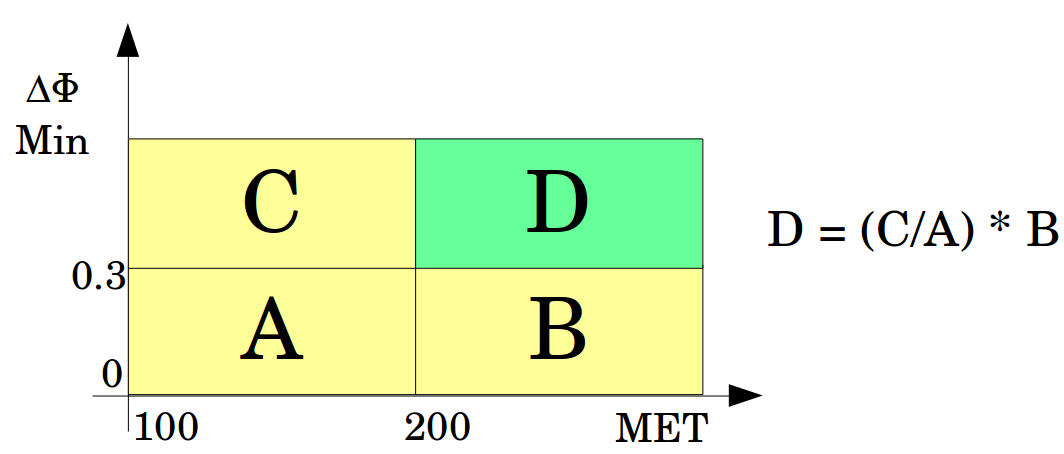
\includegraphics[width=0.48\linewidth]{../Figures/Chap3/SUSY_Photon_MET_JbJ_18Aug17/FakeMET/ABCD.png}
\caption[ABCD regions]{Definitions of various regions used in ABCD methods. Region D is signal region where background is to be estimated or validation region for zero photon sample.}
\label{fig:abcd}
\end{figure}

The ratio of high-\dphi to low-\dphi has a strong dependence as a function of \ptmiss. This dependence is accounted for by an additional correction factor using ratio, R, in low \ptmiss and high \ptmiss regions in MC. That is a factor $\kappa$ defined as \\
$\kappa$(\nj, \nb) = R(\nj, \nb) (high \ptmiss)/R(\nj, \nb)(low \ptmiss). \\
Please note that the ratio R and double ratio, $\kappa$ are binned in the bins of \nj and \nb. 

Using these values of R and $\kappa$, the performance of the method is validated using MC simulation. If the numbers R and $\kappa$ were derived using exact search region definitions, the closure would be one. Hence this validation mainly tests performance parameterization of these factors. The results of this closure tests are shown in Figure \ref{fig:qcdclosure} as a function of search bins used for this analysis. The number of \gjets and QCD multijet background events estimated using the methods (blue) closely reproduces those expected in search regions (cyan). The first bin in each \nj-\nb block corresponds to 100 $<$ \ptmiss $<$ 200~\gev control regions, where expected and predicted backgrounds exactly match by definition.

\begin{figure}[h!]
\centering
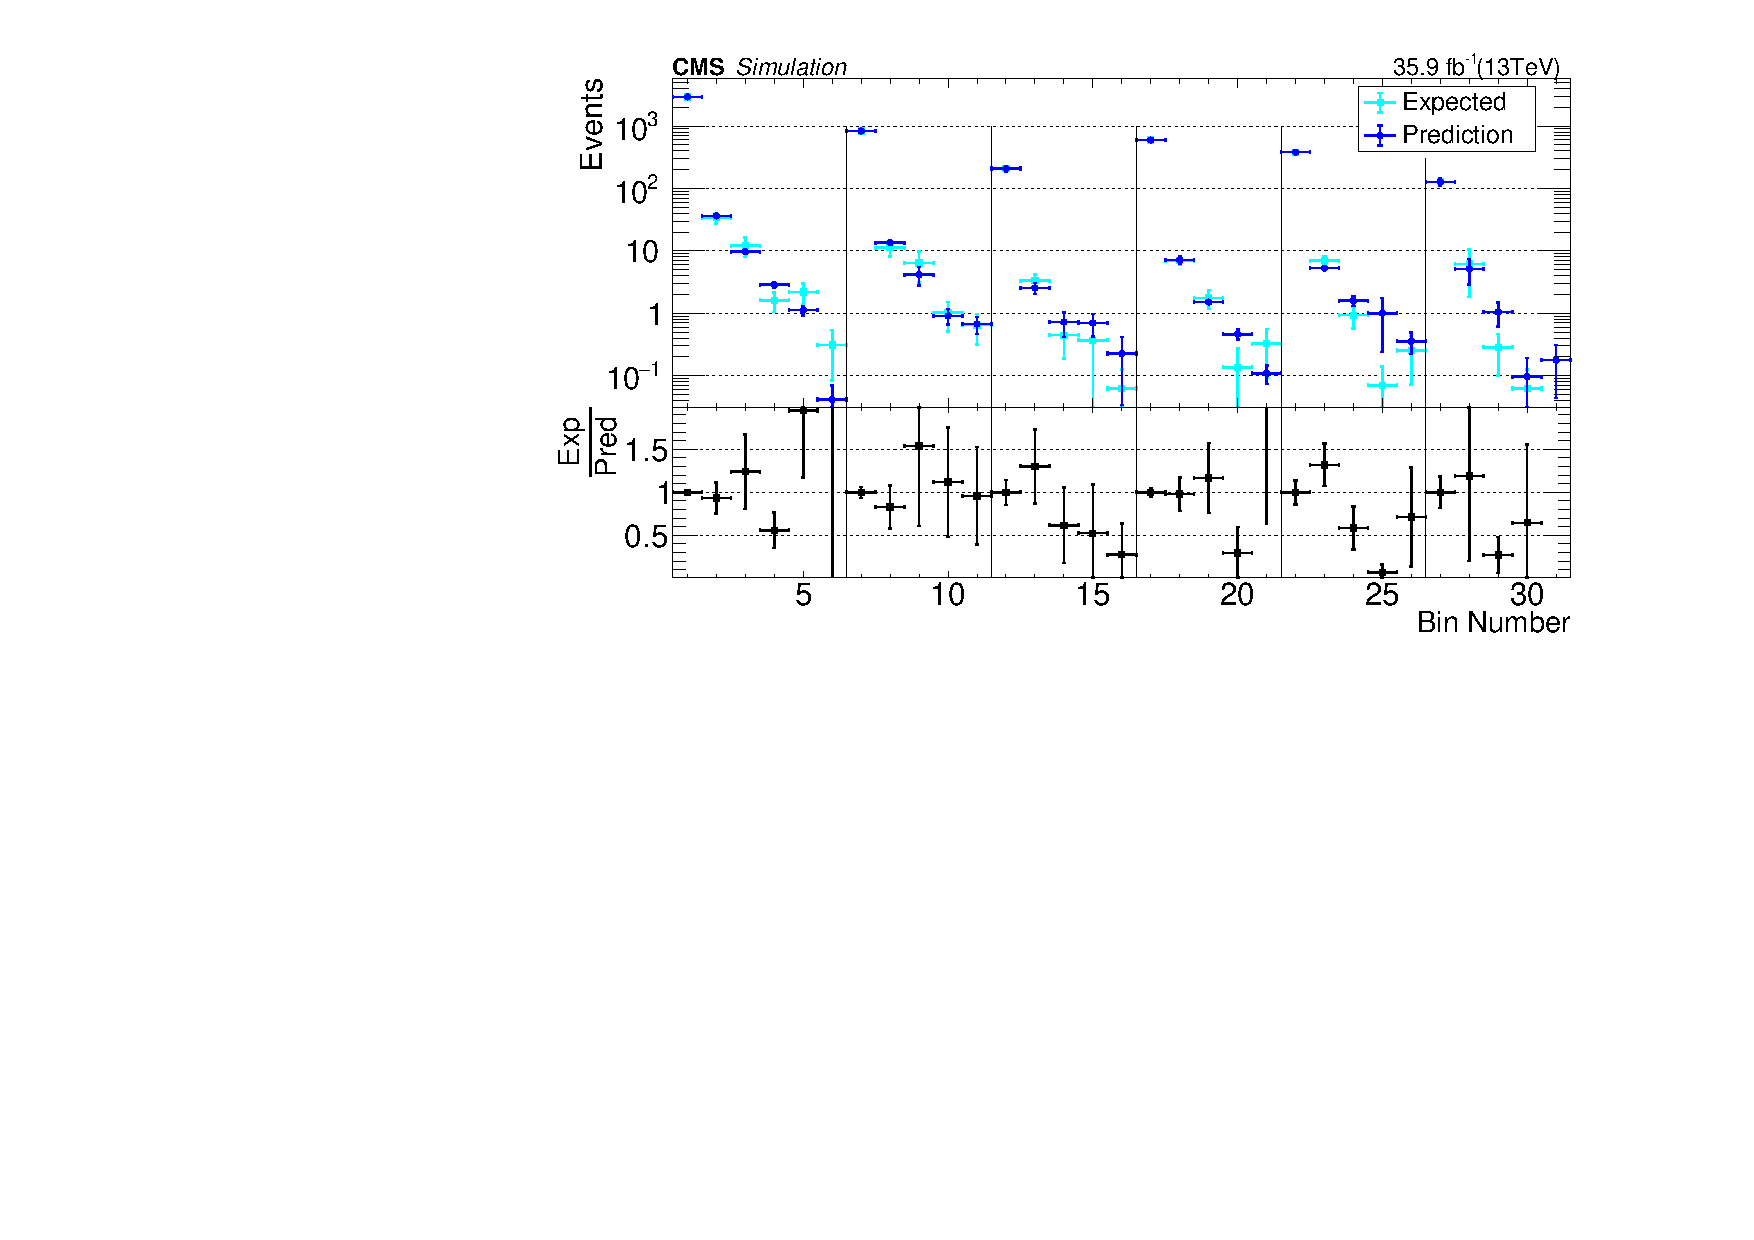
\includegraphics[width=0.85\linewidth]{../Figures/Chap3/SUSY_Photon_MET_JbJ_18Aug17/FakeMET/SBins_v4_prompt_doubleR_SRselection.pdf}
\caption[Closure for \gjets and QCD multijet]{Comparison of \gjets and QCD multijet background estimated using low-\dphi control regions taken from MC (blue) to that expected in search regions (cyan).}
\label{fig:qcdclosure}
\end{figure}

\begin{table}[h!]
\centering
\caption[Double ratio in data and MC for validation region]{Double ratio($\kappa^{\text{MC}}$) computed in the one $\gamma$ regions and ratio of high-$\dphi$ to low-$\dphi$ ($R^{data}$) obtained from data using 100 $<$ \ptmiss $<$ 200~\gev region with electroweak contribution subtracted.}
\label{tab:qcdDoubleRatioPhoton}
\begin{tabular}{c|c|c|c}
\nb & \nj  & $K^{\text{MC}}$ & $R^{data}$\\\hline\hline
\multirow{3}{*}{0} & 2 - 4   &  0.29  $\pm$  0.04   &   0.80 $\pm$  0.02 \\
   & 5 - 6   &  0.47  $\pm$  0.11   &   0.94 $\pm$  0.05 \\
   &$\geq 7$ &  0.40  $\pm$  0.11   &   1.04 $\pm$  0.17 \\ \hline
\multirow{3}{*}{$\geq 1$} & 2 - 4   &  0.24  $\pm$  0.05   &   0.65 $\pm$  0.03 \\
   & 5 - 6   &  0.34  $\pm$  0.07   &   0.91 $\pm$  0.09 \\
   &$\geq 7$ &  0.47  $\pm$  0.34   &   1.29 $\pm$  0.26 \\ \hline
\end{tabular}
\end{table}

Since the double ratio $\kappa$(\nj,\nb) used for correcting R in low and high \ptmiss regions is obtained from MC, and makes an important component of this method, it is validated using data. To define the data control sample, photon selection is inverted and events with a well identified photon are vetoed. In these zero photon events, the jet with the highest electromagnetic fraction is used as a proxy to the photon, and all baseline selection criteria are applied to the event. The jet used as proxy-photon is removed from the list of jets to avoid any double counting of the objects. With this zero photon event sample, double ratio, $\kappa$(\nj,\nb), is calculated exactly as in MC events. 

The zero photon control sample is obtained from the data collected using a combination of inclusive \HT and single jet triggers as explained in~\ref{sec:triggers}. The electroweak contribution to this sample is subtracted using event yields from the MC simulation samples. The MC event yields are corrected for the trigger efficiencies. Since these triggers achieve efficiency plateau only for \HT$>$1 TeV, the \HT$>$1 TeV region is used for validating the double ratio. The closure of this validation method in MC is shown in Figure \ref{fig:no_photon_closure}. 
\begin{figure}[h!]
\centering
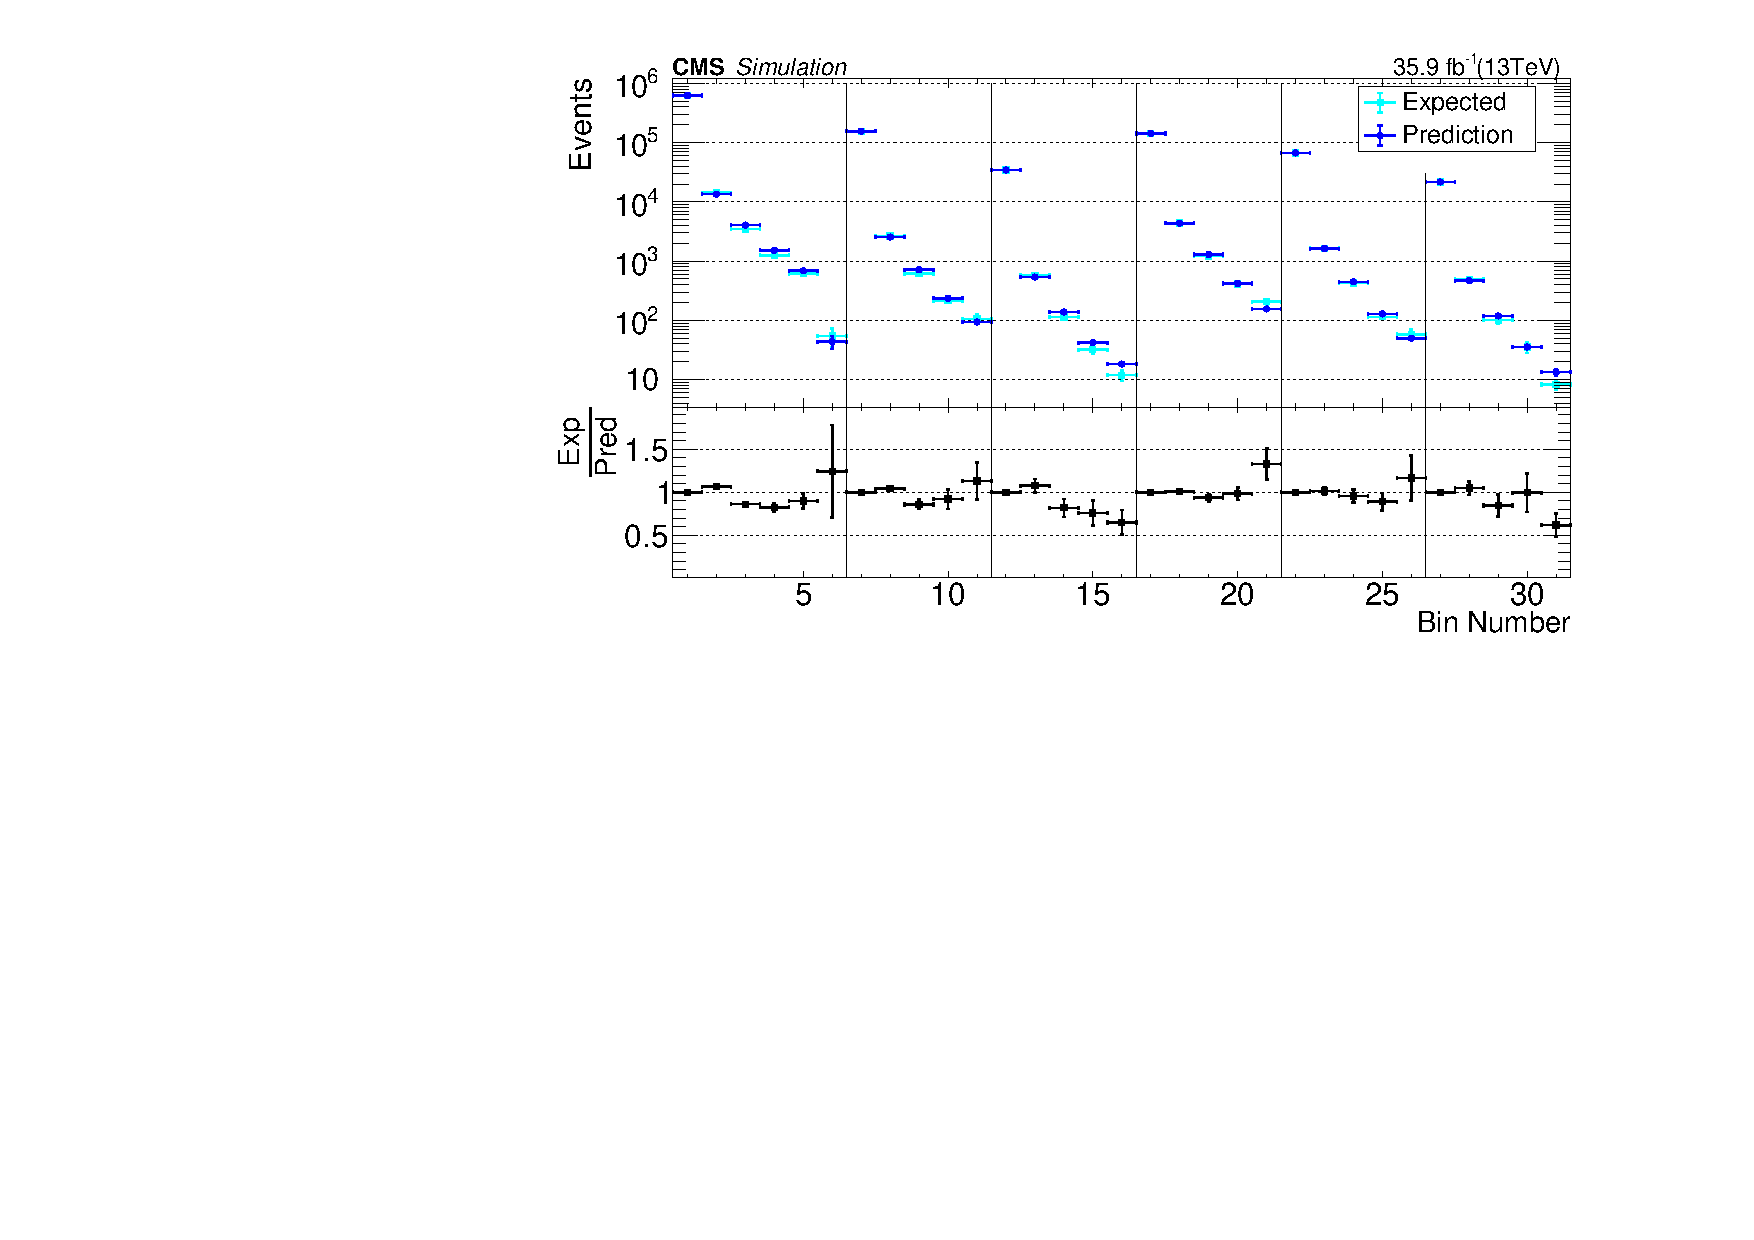
\includegraphics[width=0.85\linewidth]{../Figures/Chap3/SUSY_Photon_MET_JbJ_18Aug17/FakeMET/doubleR_ST1000.pdf}
\caption[Closure for VR]{In zero photon validation region in MC, comparison of \gjets and QCD multijet background estimated using low-\dphi control regions taken from MC (blue) to that expected in search regions (cyan).}
\label{fig:no_photon_closure}
\end{figure}

The values of double ratio, $\kappa$(\nj,\nb) obtained from zero photon validation region in data and MC are compared in Figure \ref{fig:Figure_003}.
\begin{figure}[h!]
\centering
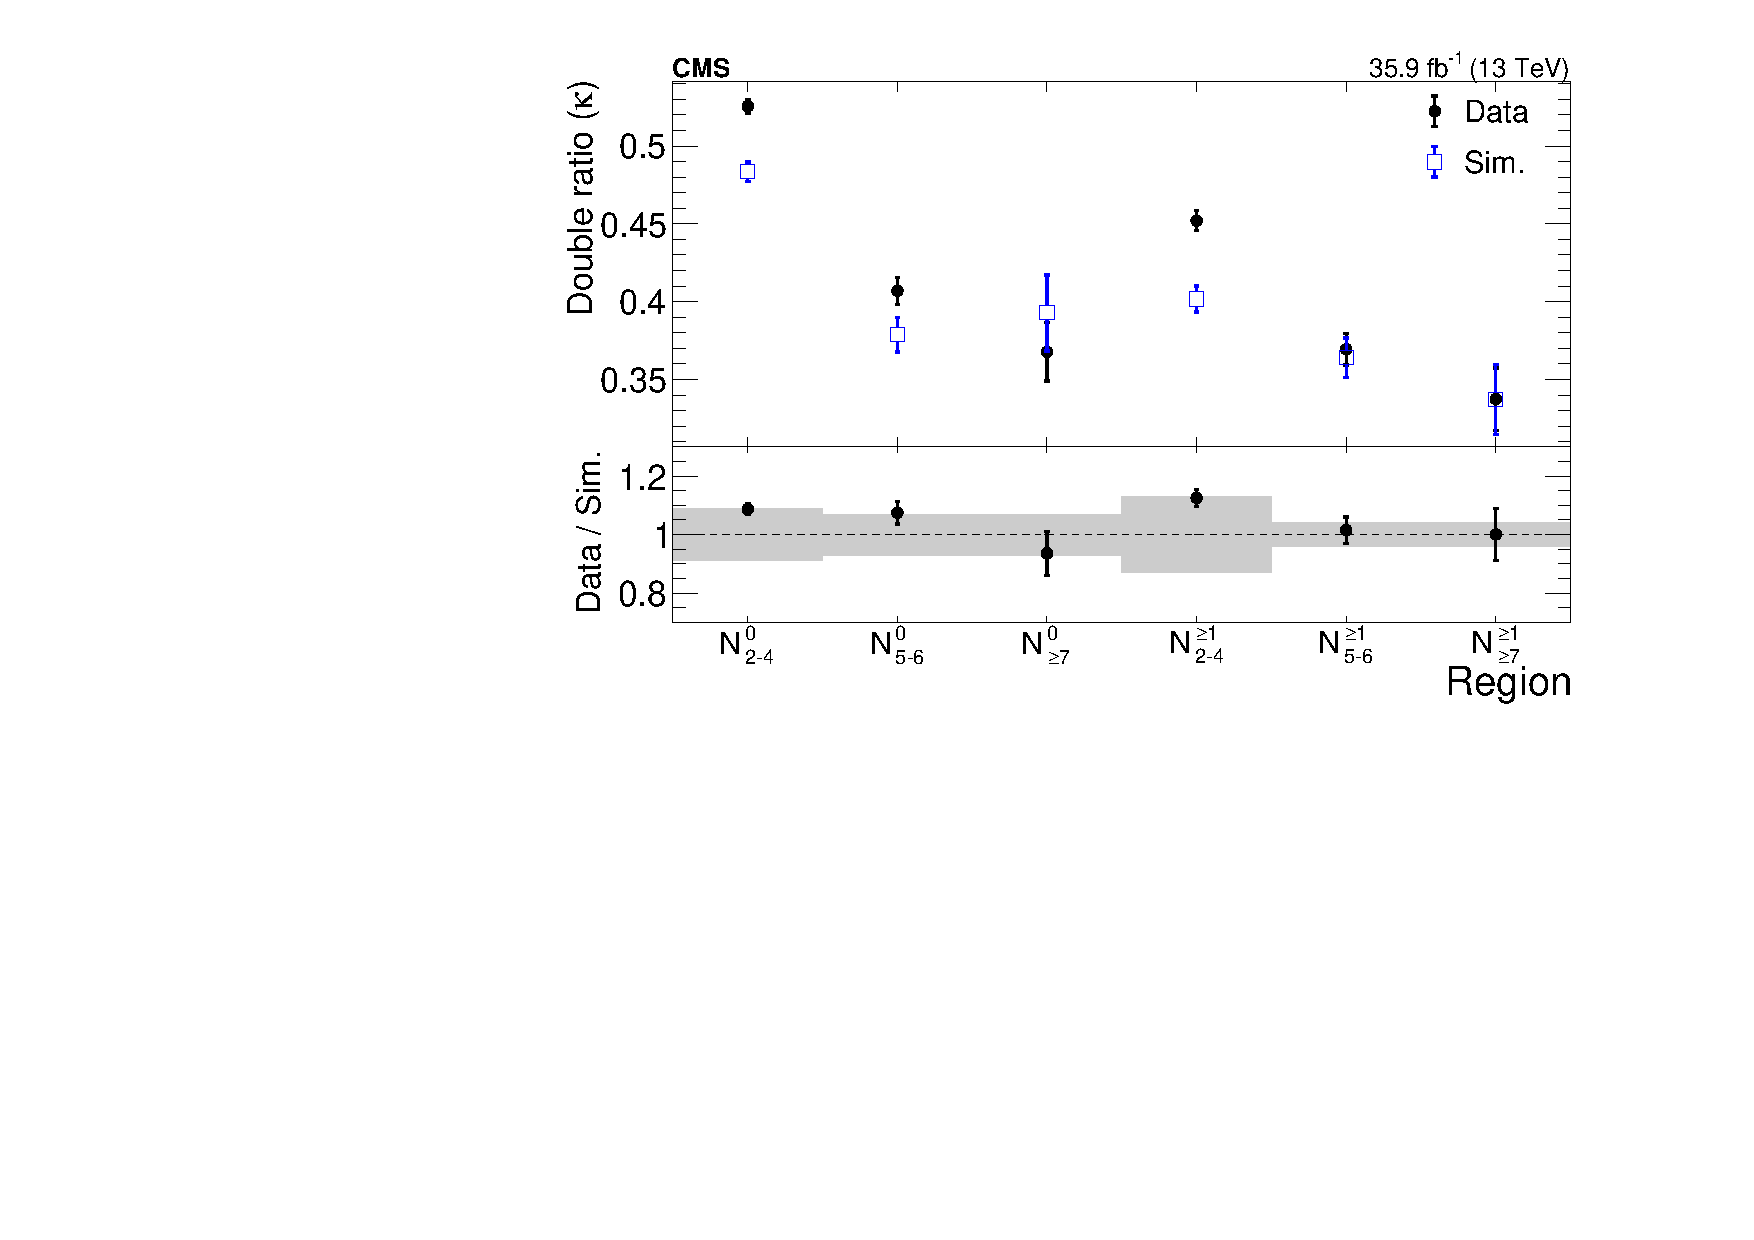
\includegraphics[width=0.8\linewidth]{../Figures/Chap3/anaPublic/Figure_003}
\caption[Double ratio validation]{The double ratio $\kappa$ in each \nj-\nb region for
zero-photon events. The filled black circles are the observed $\kappa$ values after subtracting
the electroweak contamination based on simulation. The open blue squares are the
$\kappa$ values computed directly from simulation.  The ratio is shown in the bottom
panel, where the shaded region corresponds to the systematic uncertainty in the \gjets prediction.
In the label \njb, j refers to the number of jets and b refers to the number of b-tagged jets.}
\label{fig:Figure_003}
\end{figure}

The uncertainties on predicted \gjets and QCD multijet background is dominated by statistical size of event sample in low-\dphi control region with \ptmiss $>$ 200~\gev i.e. the region B, and ranges from 6-100\%. These components of systematic uncertainties are taken uncorrelated across all bins. An additional contribution to this control region is due to uncertainties on predicted electroweak backgrounds which is subtracted from region B. This can range between 10-100\%.  Since R(\nj, \nb) = high-\dphi/low-\dphi is defined in the bins of \nj and \nb from low \ptmiss sideband region in single photon side band, statistical uncertainties on R are taken to be correlated for all bins with same \nj and \nb. The uncertainties on double ratio have two components: (a) difference between $K_{0\gamma}$ in data and MC, and (b) statistical uncertainty on $K_{0\gamma}^{\text{MC}}$. These two contributions are added in quadrature to assign the systematic uncertainties which are also taken fully correlated for all bins with same \nj and \nb.
The final predictions of \gjets and QCD multijet processes is shown in \ref{tab:qcdPrediction}.

